Computer aided detection (CAD) is a clinically proven technology that increases the detection of clinical signs and diseases by assisting the doctors in decreasing observational oversights. The more recent clinical introduction of CAD to assist doctors in the detection of pulmonary signs and diseases will likely be followed by the development, clinical trials validation, regulatory approval and commercialization of a variety of CAD applications in diagnostic imaging. \cite{Castellino2005}
\\ \\
These kinds of software are being used in all fields of medicine but because of the nature of the data itself it is more used in areas where the clinical diagnosis is mostly made by using visual tools, like radiology for example. The computer analyses the image and symptomatic data and outputs a likelihood percentage to aid the doctor in his/her diagnosis.
\\ \\
Nonetheless, making a diagnosis based on images of a patient is often not an easy task. The idea of using computers to help, and possibly improve the interpretation of medical images is therefore very appealing. The first reference to the term computer-aided diagnosis that I have found is in a paper from 1963 by G.S. Lodwick, in Investigative Radiology 1(1):72-80 entitled "Computer-aided diagnosis in radiology. A research plan." \cite{Lodwick1966}

\section{Similar solutions}

There are many companies investing in this field of aided diagnostics, but when analyzing it just for the ones who are focusing on tuberculosis, we can say that EPCON has two main competitors in the market:

\begin{itemize}

\item
\textbf{Qure.ai} from the United States, which has a product named \textbf{qXR} that detects abnormal chest X-rays, then identifies and localizes 15 common abnormalities and screens for tuberculosis. It is used in public health screening programs and was trained with over a million curated X-rays and radiology reports, making it hardware-agnostic and robust to variations in X-ray quality. \cite{QureAI}

\item 
\textbf{Delft Imaging} from the Netherlands, that developed \textbf{CAD4TB} in order to help (non-expert) readers detect tuberculosis more accurately and cost-effectively through the speed of digital X-rays combined with deep learning and remote expertise. \cite{DelftImaging}
	
\end{itemize}

All these technologies have a big focus on computer aided-diagnosis, whoever, we were not developing the CAD AI system ourselves, but rather using the one already built and tested provided by EPCON. Our job was to build an application wrappers around it to make it user friendly and usable for the web and for mobile.

\section{Web application development context}

The way we develop web application has come along way since its beginnings.
\\ \\
During the \textbf{early 90s} was the era of the static HTML pages, where web pages were text documents and only later it was possible to add styles, images, audio and video files.
\\ \\
Around \textbf{1995} the JavaScript language was presented, which made the web pages faster and added the possibility of having dynamic client content and elements on the web pages.
\\ \\
In the year \textbf{1996} Flash was introduced by Macromedia, which allowed to enrich the web pages with interactive animations using a programming language called ActionScript. This allowed for an explosion of interactive web video games on the world wide web.
\\ \\
Around \textbf{2006} there started to be a shift from static to dynamic web applications with the introduction of jQuery, which made DOM manipulation way easier and browser consistent and with the introduction of Ajax technology, which enabled the client (in this case the browser) to make asynchronous requests to REST APIs. During this time it was also introduced the the notion of responsive web design, where developers would build applications that would scale depending on the window width, making it available for smaller screens on mobile and larger screens on desktop, writing the application just once, instead of having two separate versions for mobile and desktop users.
\\ \\
During \textbf{2011} there was a big leap forward for web development because of the introduction of the HTML5 spec. It improved widely the standards, supporting most types of multimedia to be present on the web and allowing to create web applications that are independent from browsers and platforms. The introduction of HTML5 marked the beginning of the decline in the use of Flash for interactive content on web pages. Around this time some web application frameworks started to become popular and widely used, most notably Backbone and Ember.js.
\\ \\
From around \textbf{2016} frameworks like Angular, React and Vue started to emerge and the concept of progressive web application was born. Using the latest browser APIs, like notification, geo-location, and service workers, web applications could behave almost identical to native apps.
\\ \\
Nowadays the development of client-side web applications is dominated by \textbf{React} and \textbf{Vue}, followed by \textbf{Angular}. Concepts like server-side rendering, static HTML generation and posterior hydration with JavaScript and offline usage using service workers have been widely adopted and standardized.

\\ \\
\begin{figure}[H]
	\centering
	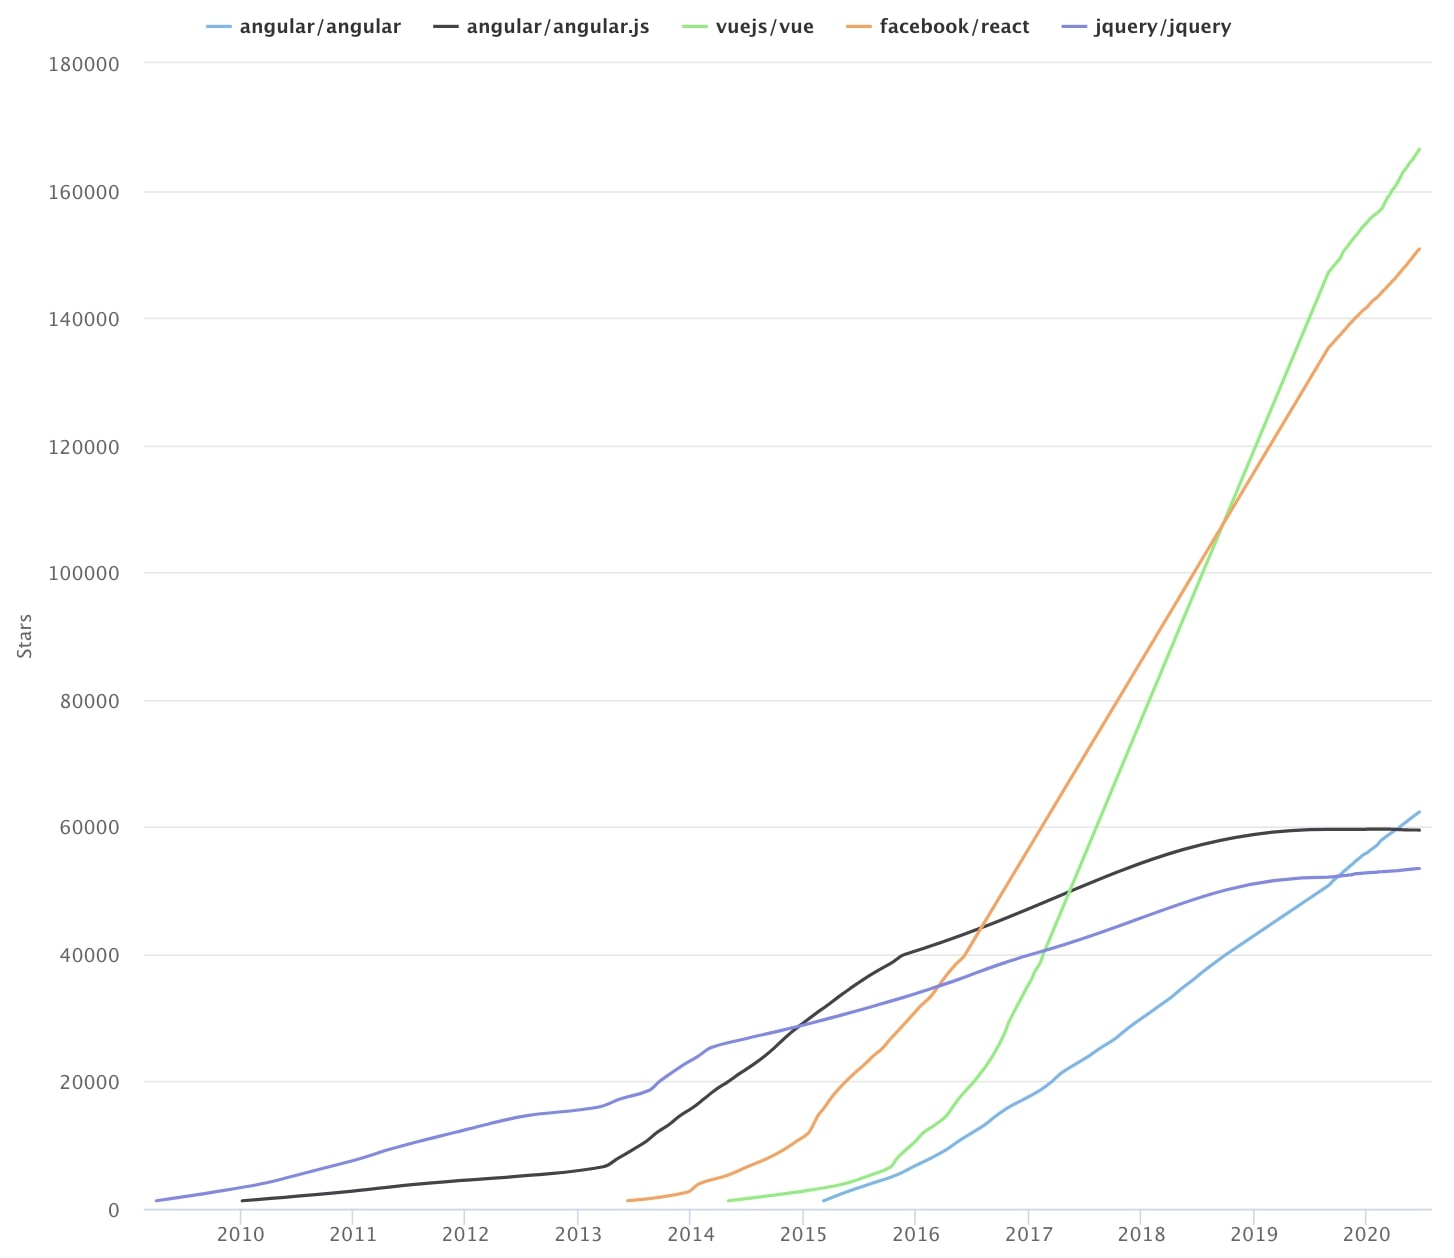
\includegraphics[width=1.0\linewidth]{pesti-report/images/web-app-frameworks-graph.jpg}
	\caption{Web application framework popularity by GitHub stars}
	\label{fig:web-app-frameworks-graph}
\end{figure}
\\

\section{Mobile application development context}

The state of the development of mobile applications has been evolving since its conception and it still didn't grew to a completely mature point as progresses are being made still every single day.
\\ \\
In the context of mobile applications we can divide them into two distinct groups: \textbf{native applications} and \textbf{hybrid applications}.
\\ \\
A \textbf{native application} is a software which has been developed to perform some specific task on particular environment or platform, built using a SDK for a certain software framework, hardware platform or operating system. For example, Android applications are build using the Java development kit and Kotlin or Java, iOS applications using the iOS SDK, Swift and Objective-C and Windows applications using the .NET frameworks and the C# language.
\\

\begin{center}
 \begin{tabular}{||c c||}
 \hline
 Operating System & Frameworks and Languages \\ [0.5ex]
 \hline\hline
 Android & JDK, Kotlin, Java  \\
 \hline
 iOS & iOS SDK, Swift, Objective-C  \\
 \hline
 Windows & .NET, C#  \\
 \hline
\end{tabular}
\end{center}

 
\\ \\
An \textbf{hybrid application} has some similarities to the native apps but also some differences. It can be downloaded from the platforms app store just like native apps do, it can get access to most of the native platform features and it's performance can become close to the native app. The major difference is that with an hybrid app the developers can write code just once and publish it in all platforms. The are advantages and disadvantages in deciding to build an hybrid app instead of a native app.
\\ \\
\textbf{Advantages of hybrid apps:}

\begin{itemize}
\item
Typically faster to develop
\item 
Unified development of having a single code base
\item 
Less expensive to build and maintain
\item
Ability to target a wider user pool without much effort

\end{itemize}

\\ \\
\textbf{Disadvantages of hybrid apps:}

\begin{itemize}

\item
Hybrid UI feels less responsive to users
\item 
Indirect access to device hardware and software APIs, usually accessed through framework wrappers
\item 
Worse performance

\end{itemize}

As of today, there are three popular frameworks for creating hybrid mobile applications: \textbf{Ionic}, \textbf{React Native} and \textbf{Flutter}.
\\ \\

\begin{figure}[H]
	\centering
	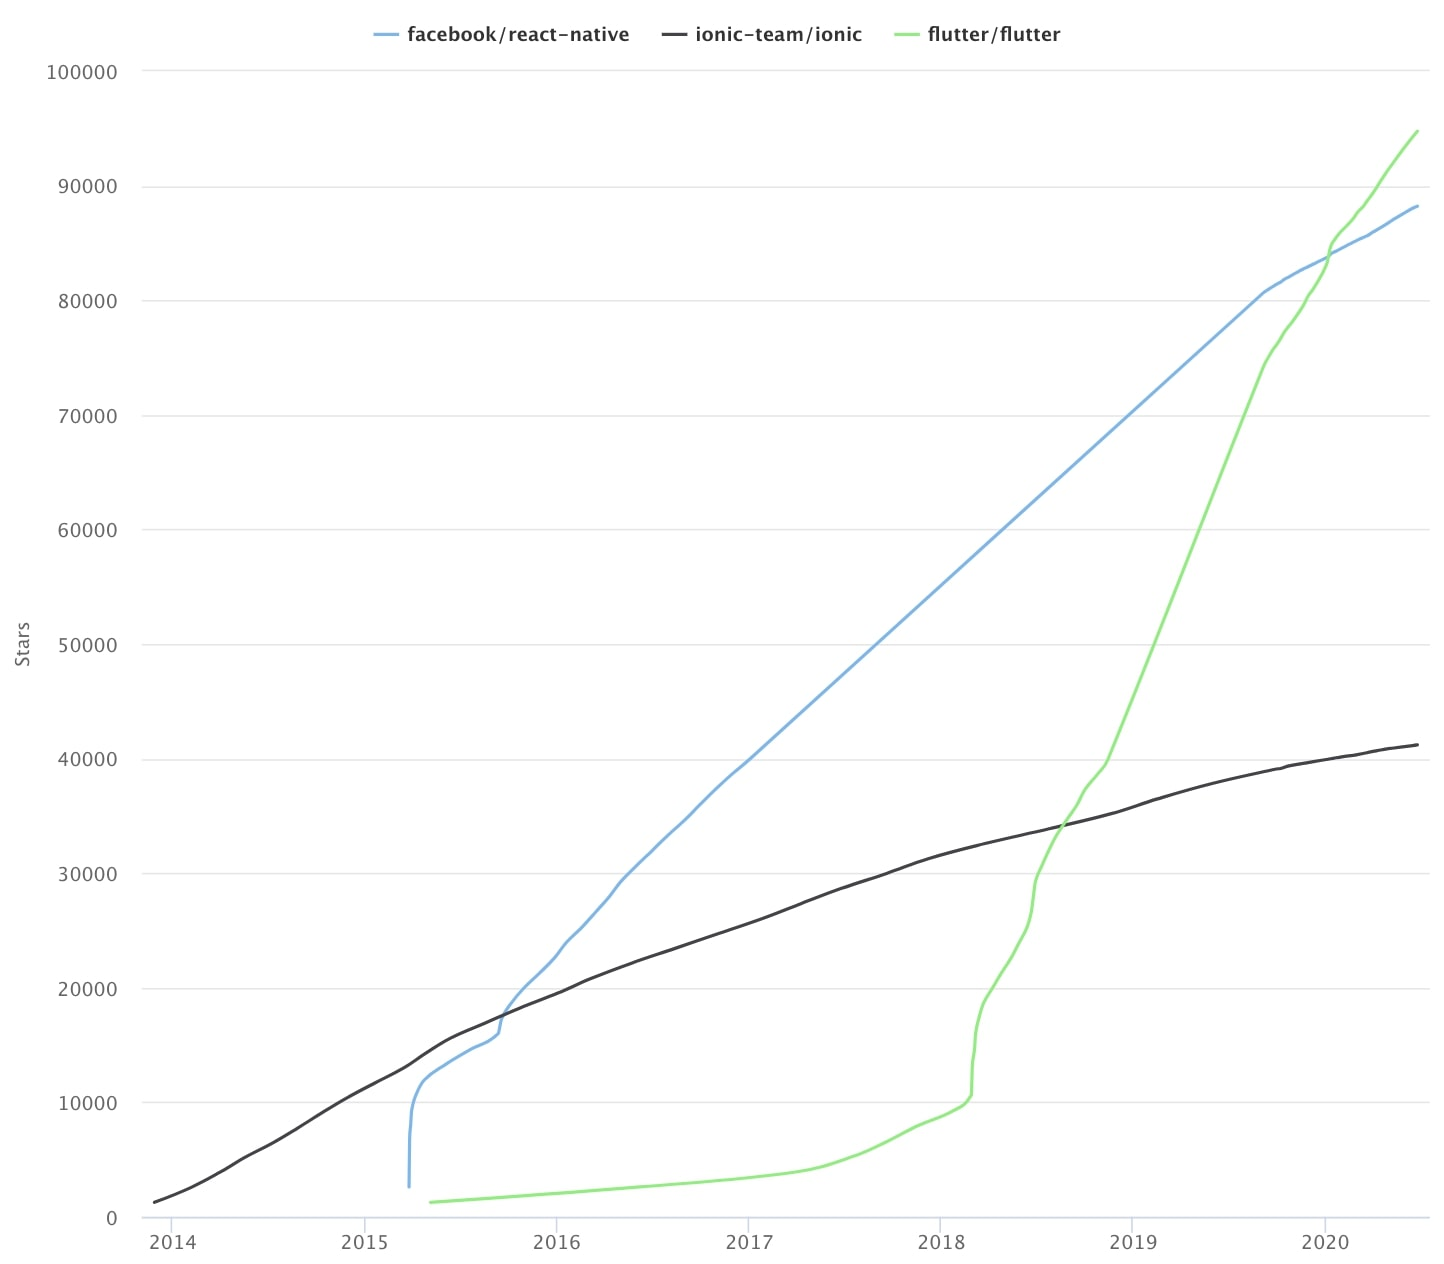
\includegraphics[width=1.0\linewidth]{pesti-report/images/mobile-hybrid-frameworks-graph.jpg}
	\caption{Mobile hybrid framework popularity by GitHub stars}
	\label{fig:mobile-hybrid-frameworks-graph}
\end{figure}


\textbf{Ionic} is a framework that allows developing applications for iOS and Android. It embeds the application inside a browser without the navigation options (or WebView) that can be run as a standalone application on any platform. \cite{IonicGitHub}
\\ \\
\textbf{React Native} uses a very different approach to browser-based described above. Instead of rendering content in a WebView or the mobile web browser, the content is rendered with native OEM components provided by the platform. JavaScript is still used for the application logic to be able to re-use the same logic across platforms, and the rendering, which is the most performance-sensitive part, is done with native components for increased performance. \cite{ReactNativeGitHub}
\\ \\
\textbf{Flutter} is the latest and more trending nowadays. It was developed by Google and uses a programming language named Dart, which is also maintained by Google. It provides very good and fast tools to work, build and run the code and it maintains solid consistency between all platforms. \cite{FlutterGitHub}